
During the dedicated experiment that took place in the SPS
in 2018 with the CCs, the measured emittance
growth was found to be a factor four (on average) lower than
expected from the theory (see Section~\ref{sec:meas_2018_vs_theory}). The reason for this discrepancy remained unresolved for some time, as detailed follow-up studies (see Chapter~\ref{Ch:investigating_discrepancy}) investigated and excluded a number of possible explanations for the discrepancy.
It was recently found, that the beam transverse impedance, which is not included in the theory~\cite{PhysRevSTAB.18.101001} used for the comparison with the measurements may impact the noise-induced emittance growth and explain the experimental observations. Here, the damping mechanism from the beam transverse impedance is investigated as observed in detailed PyHEADTAIL simulations.

The structure of this chapter is as follows:




\section{SPS transverse impedance model}\label{sec:sps_impedance_model}
The PyHEADTAIL studies presented in this chapter are performed including the detailed transverse impedance model of the SPS machine~\cite{sps_impedance_model_git}. This model has been developed through a combination of theoretical computations, electromagentic simulations and was benchmarked with beam-based measurements~\cite{Salvant:1274254, Zannini:1561199, Salvant:1271349, Zannini:2141779}. 
It includes the contributions from all the individual elements in the SPS lattice i.e. the resistive wall, the indirect space charge, the kickers, the RF cavities (200\,MHz and 800\,MHz), the step transitions and the horizontal and vertical beam position monitors~\cite{Zannini:2141779}. As discussed in  Section~\ref{subsec:pyheadtail}, the model needs to represent the global impedance of the full machine. Thus, the total impedance is obtained by summing up the impedance of each element weighted with the beta function at its location and by dividing the sum by the average beta function of the SPS. For the Q26 optics the average horizontal and vertical beta functions are 42.09\,m and 42.01\,m respectively.
%https://indico.cern.ch/event/299470/contributions/686509/attachments/564150/777102/LIUSPS_transverse_imp_5.pdf
% The Wall contribution included both the resistive wall and the indirect SC.
Figure~\ref{fig:sps_impedance_model_H_V} shows the complete transverse impedance model of the SPS machine with the disentangled dipolar (blue) and quadrupolar (orange) terms to be plotted seperetaly. 

% Plot figures: /eos/user/n/natriant/Project_thesis/plot_wakefields_impedances_SPS
\begin{figure}[!ht]
    \centering
    \begin{subfigure}[t]{0.45\textwidth}
        \centering
        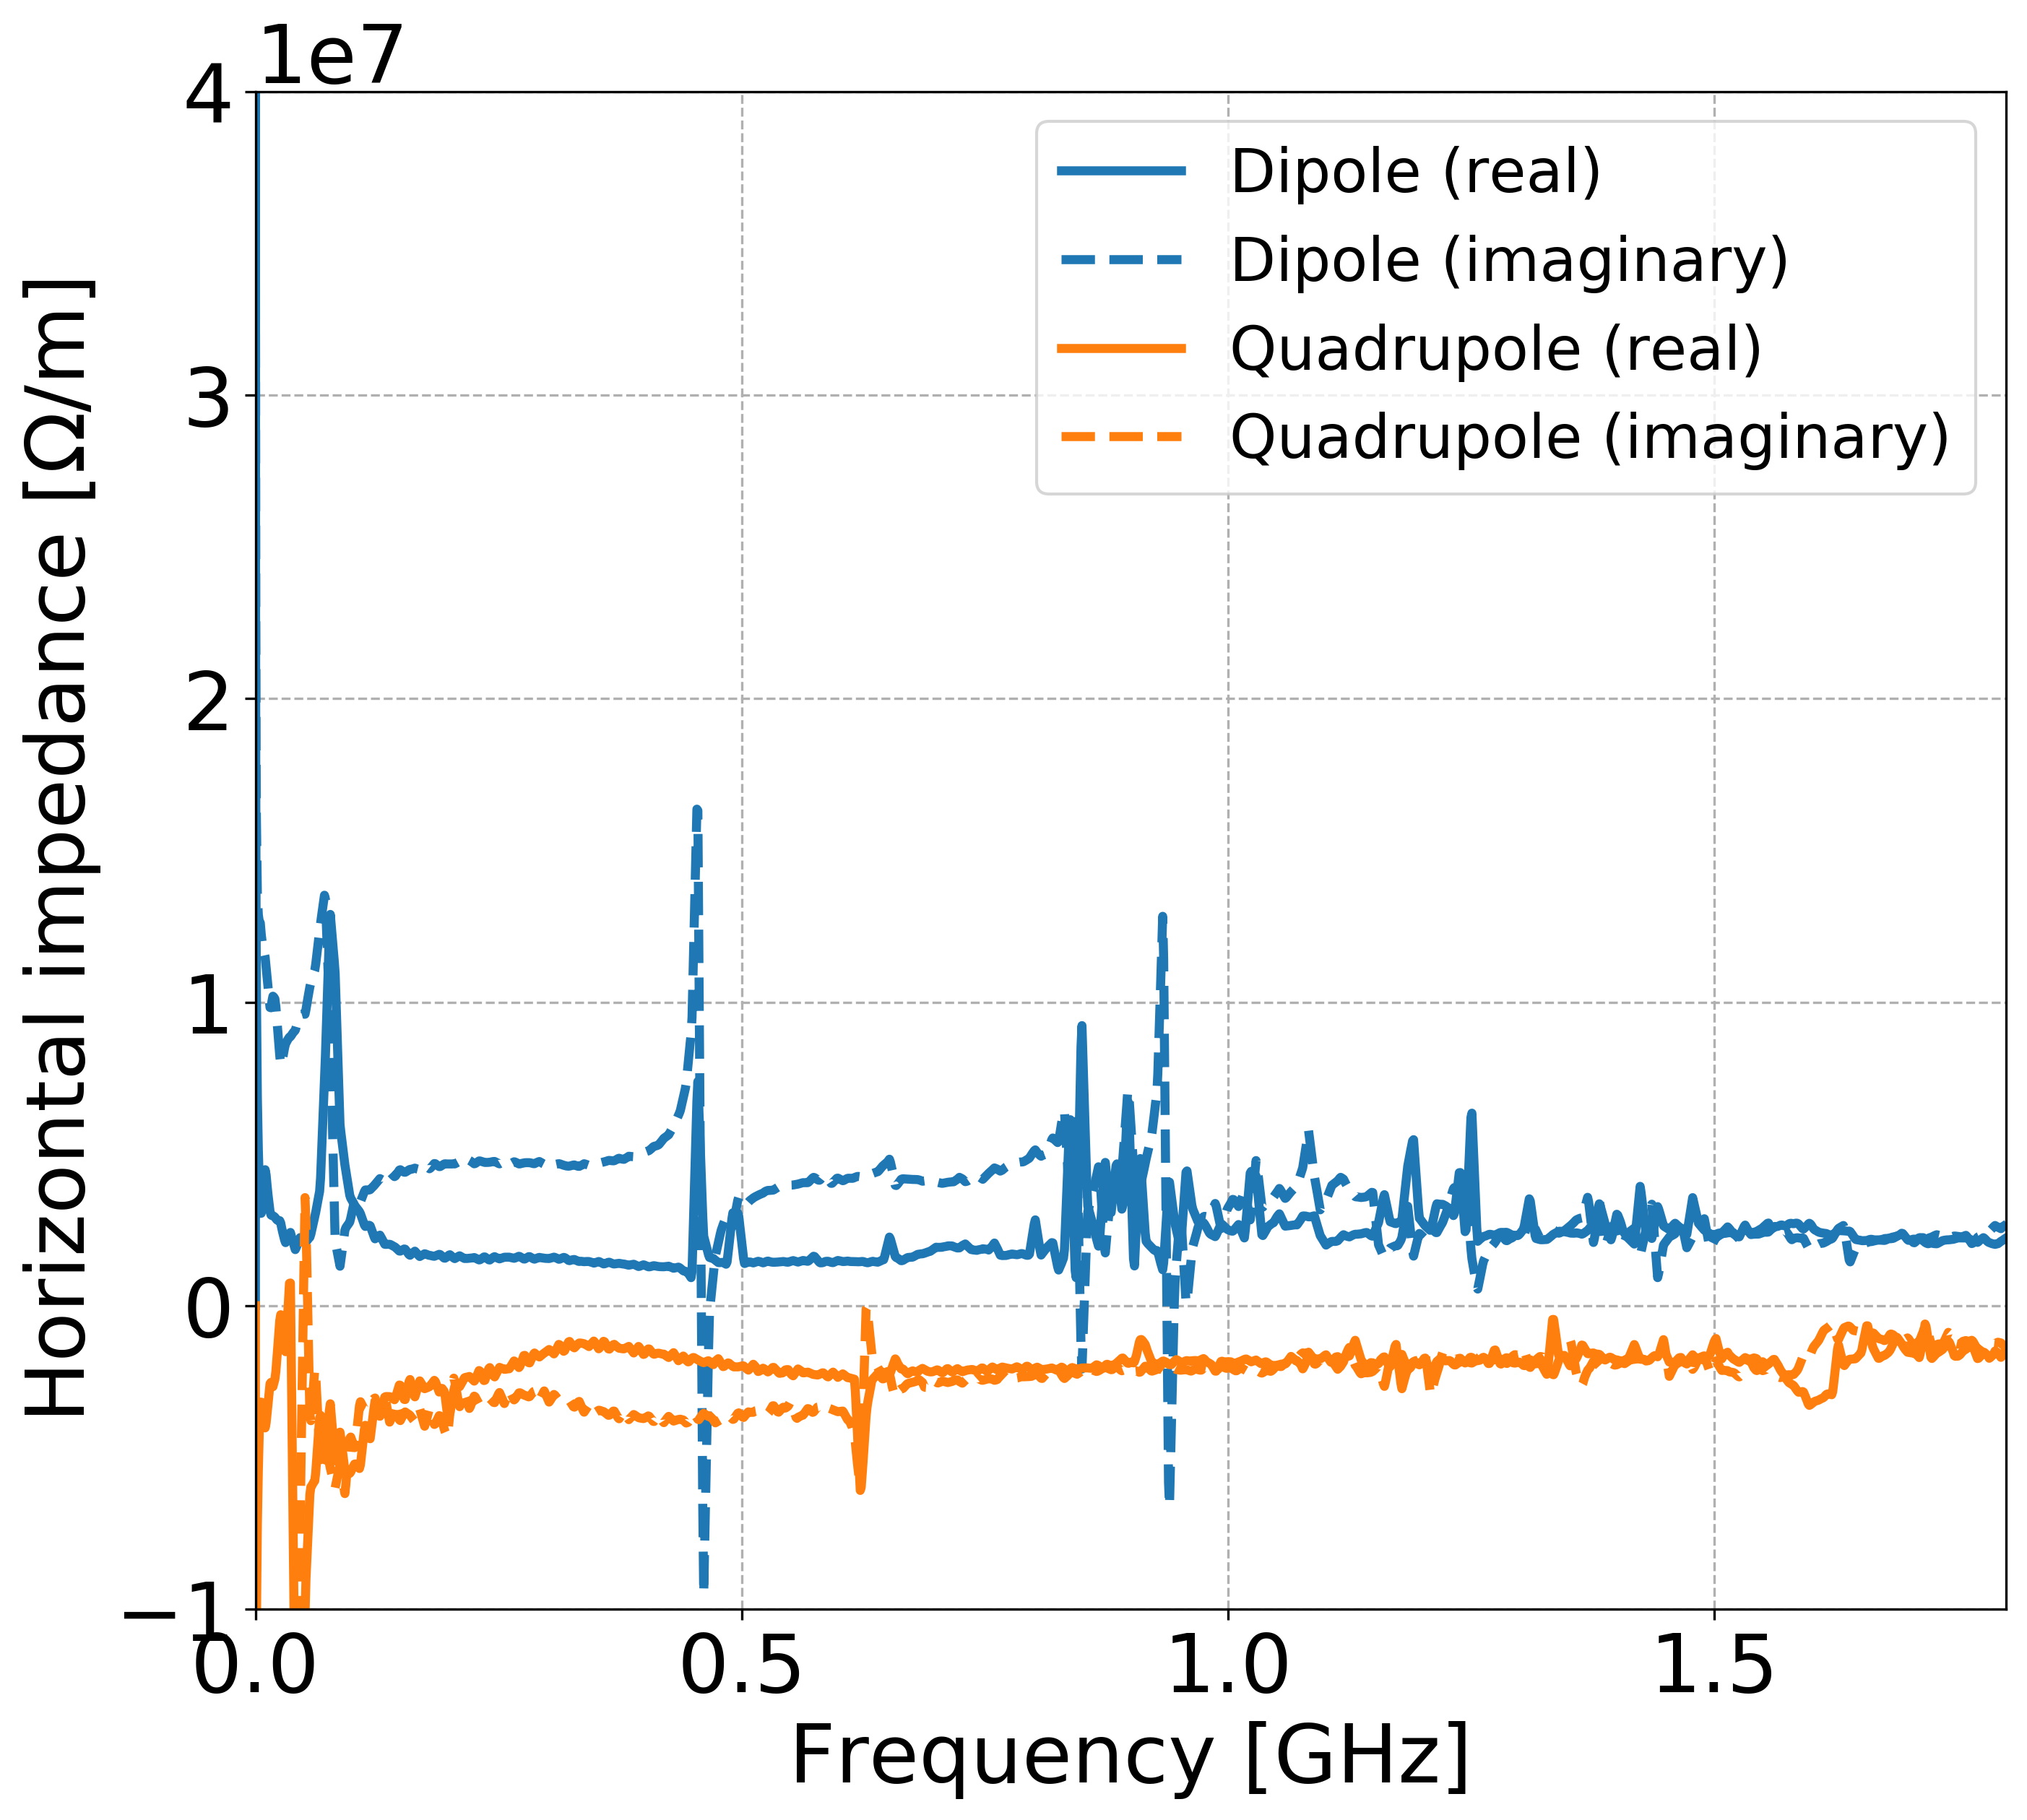
\includegraphics[width=1\textwidth]{images/Ch7/Q26_complete_SPS_model_impedance_H_plane.png}
        %\caption{$y=\sin(2 \pi f t),\ f=50$ Hz}
        %\label{fig:add_label_here}
    \end{subfigure}
    \hfill
    \begin{subfigure}[t]{0.45\textwidth}
        \centering
        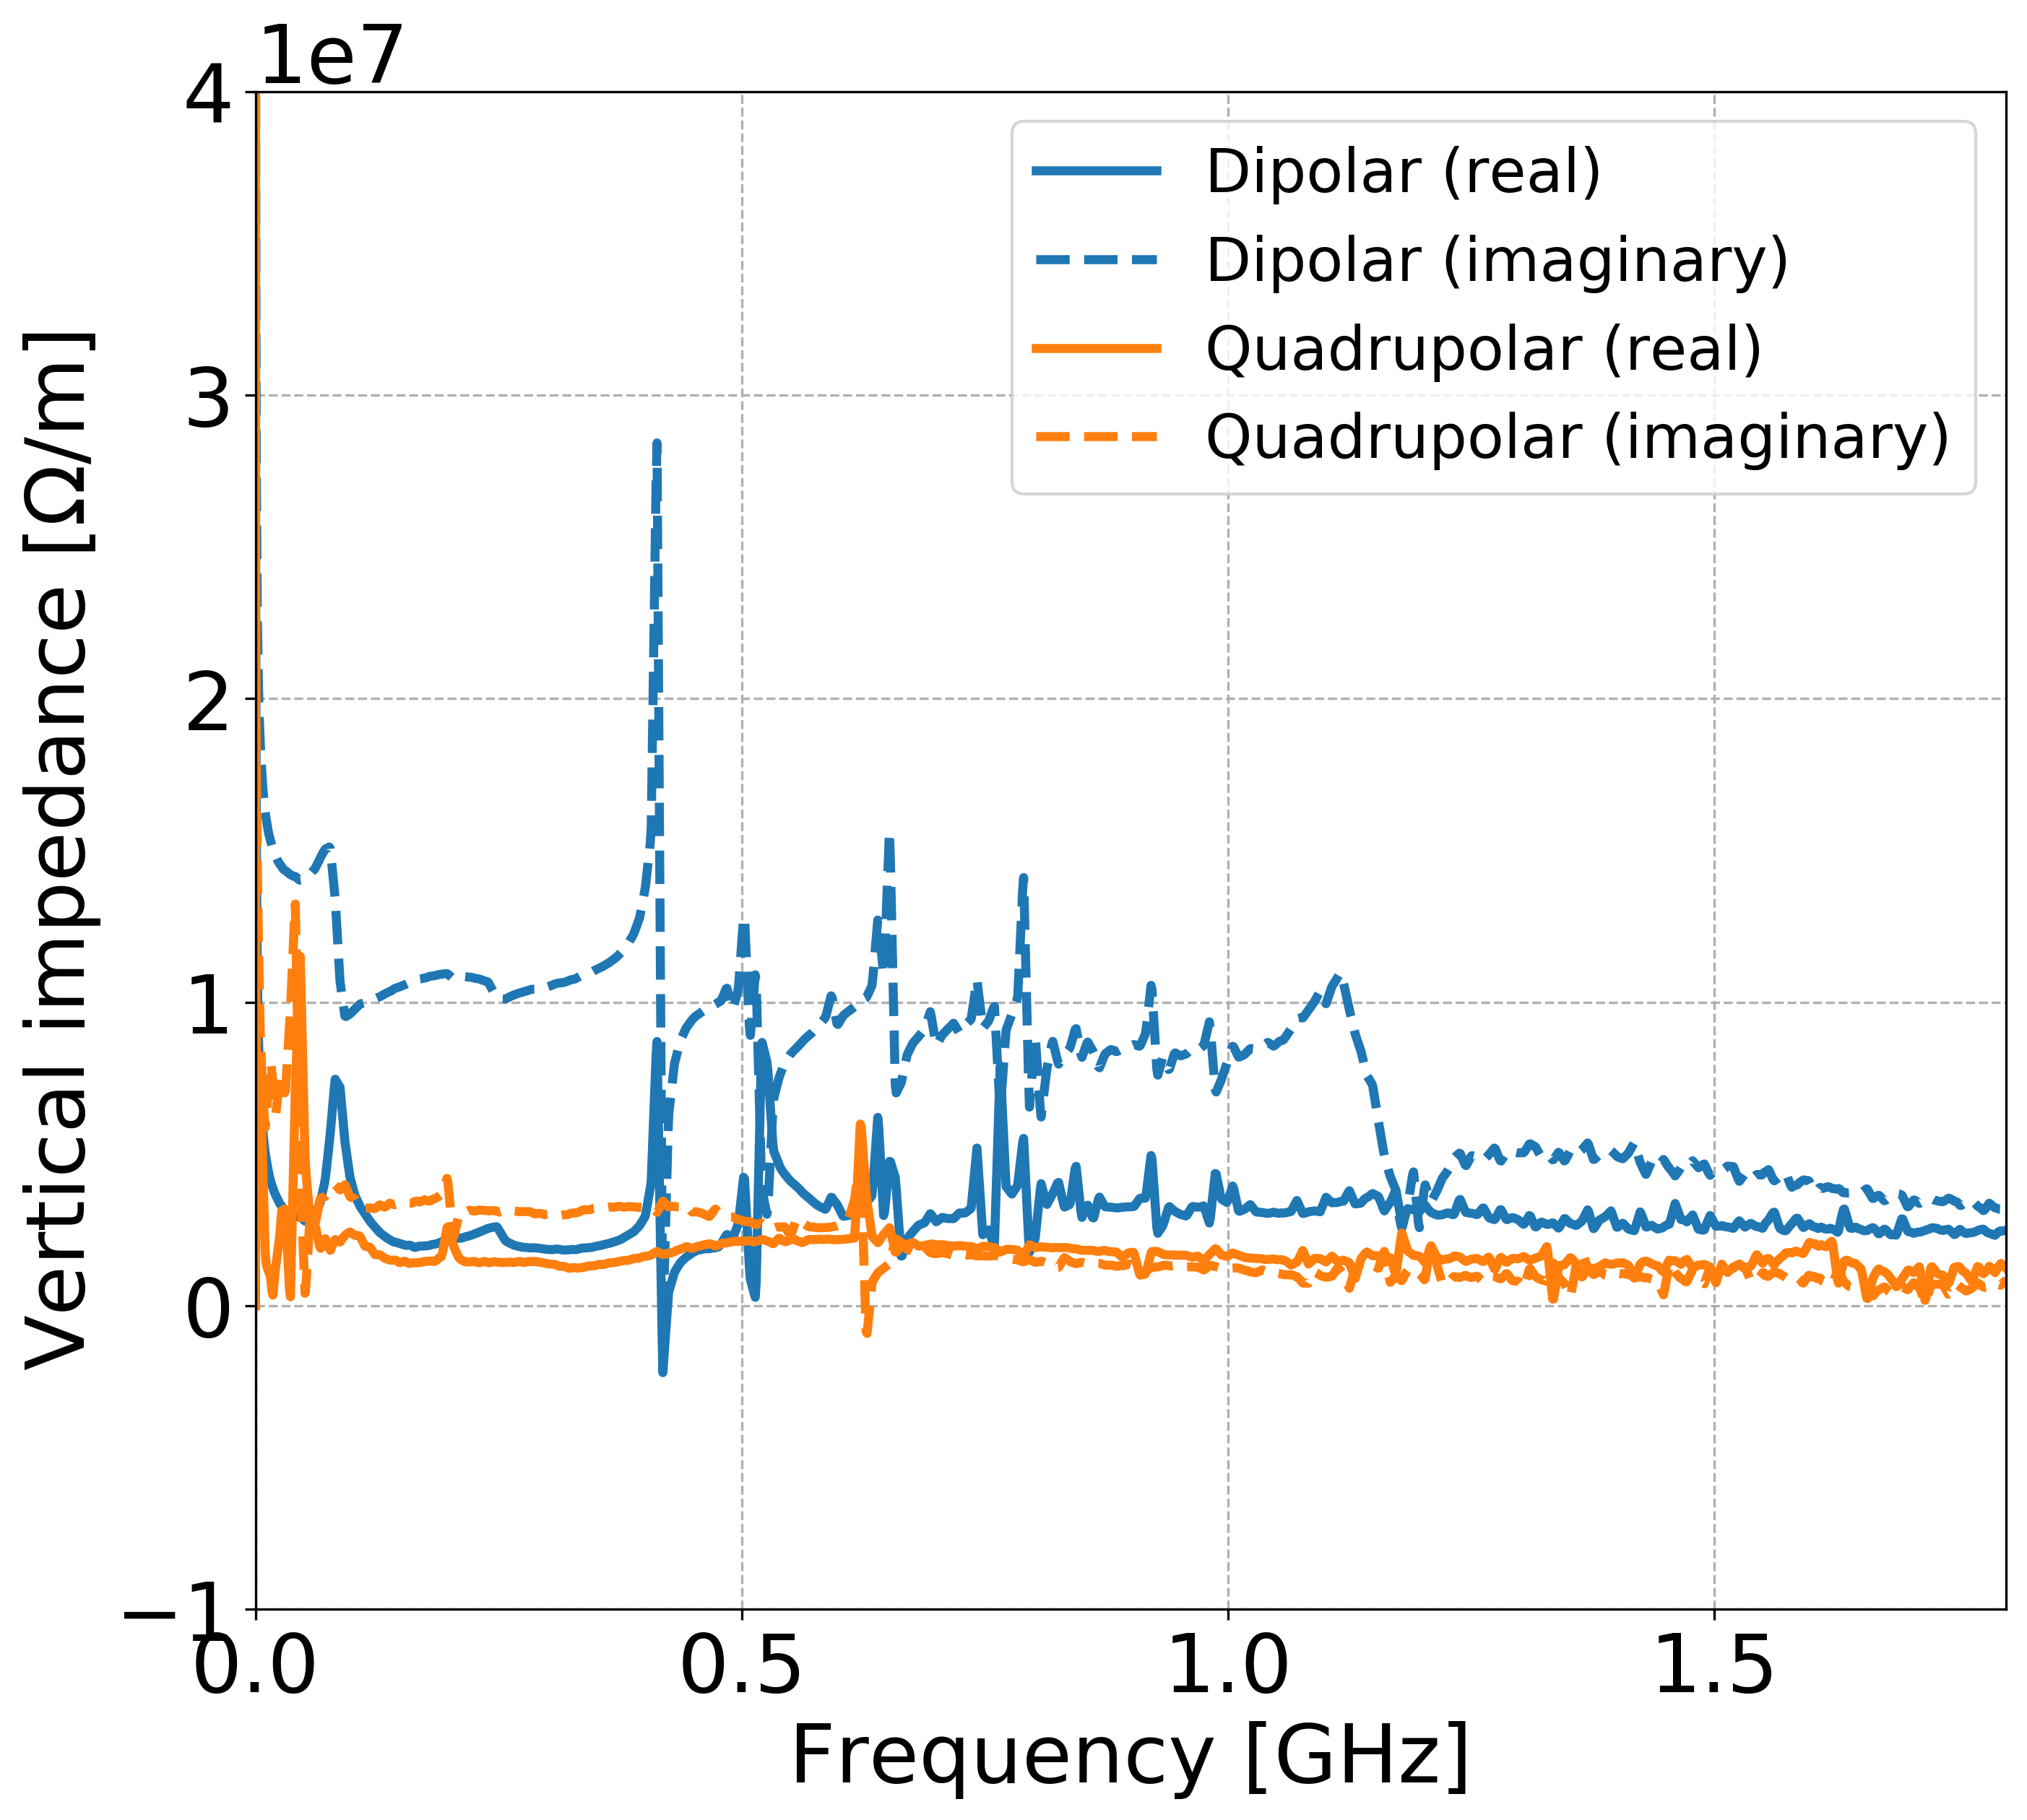
\includegraphics[width=1\textwidth]{images/Ch7/Q26_complete_SPS_model_impedance_V_plane.png}
        %\caption{Discrete Fourier transform}
        %\label{fig:add_label_here}
    \end{subfigure}
    \hfill
     \caption{Horizontal (left) and vertical (right) impedance model of the SPS. The model is available in the public gitlab repository of Ref.~\cite{sps_impedance_model_git}.} % bunch passage
     \label{fig:sps_impedance_model_H_V}
 \end{figure}

 The contributions from the wall, the kickers and the step transitions are visible at the low freqencies (up to $\sim$ 0.4\,GHz). The impedance of the RF cavities and the beam position monitors (BPMs) corresponds results to the peaks observed between $\sim$ 0.4-1\,GHz. 
%https://indico.cern.ch/event/299470/contributions/686509/attachments/564150/777102/LIUSPS_transverse_imp_5.pdf %For a clearer picture, it is worth mentioning that at low freqencies (up to $\sim$ 0.4\,GHz) the impedance is mainly from the wall the kickers and the step transitions. The peaks between $\sim$ 0.4-1\,GHz appear due to the RF cavities and the beam position monitors.
%https://indico.cern.ch/event/299470/contributions/686509/attachments/564150/777102/LIUSPS_transverse_imp_5.pdf

\normalsize{\textbf{Wake functions}}\\
As already discussed in Section~\ref{subsec:pyheadtail}, in order to include the impedance effects in PyHEADTAIL simulations the real-value wakefields in time domain are used. The wakefield kicks are computed as a convolution of the wake function with the moments of each particle. The total transverse dipolar (blue) and quadrupolar (orange) wake functions for both planes of the SPS can be found in the gitlab repository of Ref.~\cite{sps_impedance_model_git} and they are plotted in Fig~\ref{fig:sps_wakefunctions_model_H_V}.

% Plot figures: /eos/user/n/natriant/Project_thesis/plot_wakefields_impedances_SPS
 \begin{figure}[!ht]
    \centering
    \begin{subfigure}[t]{0.45\textwidth}
        \centering
        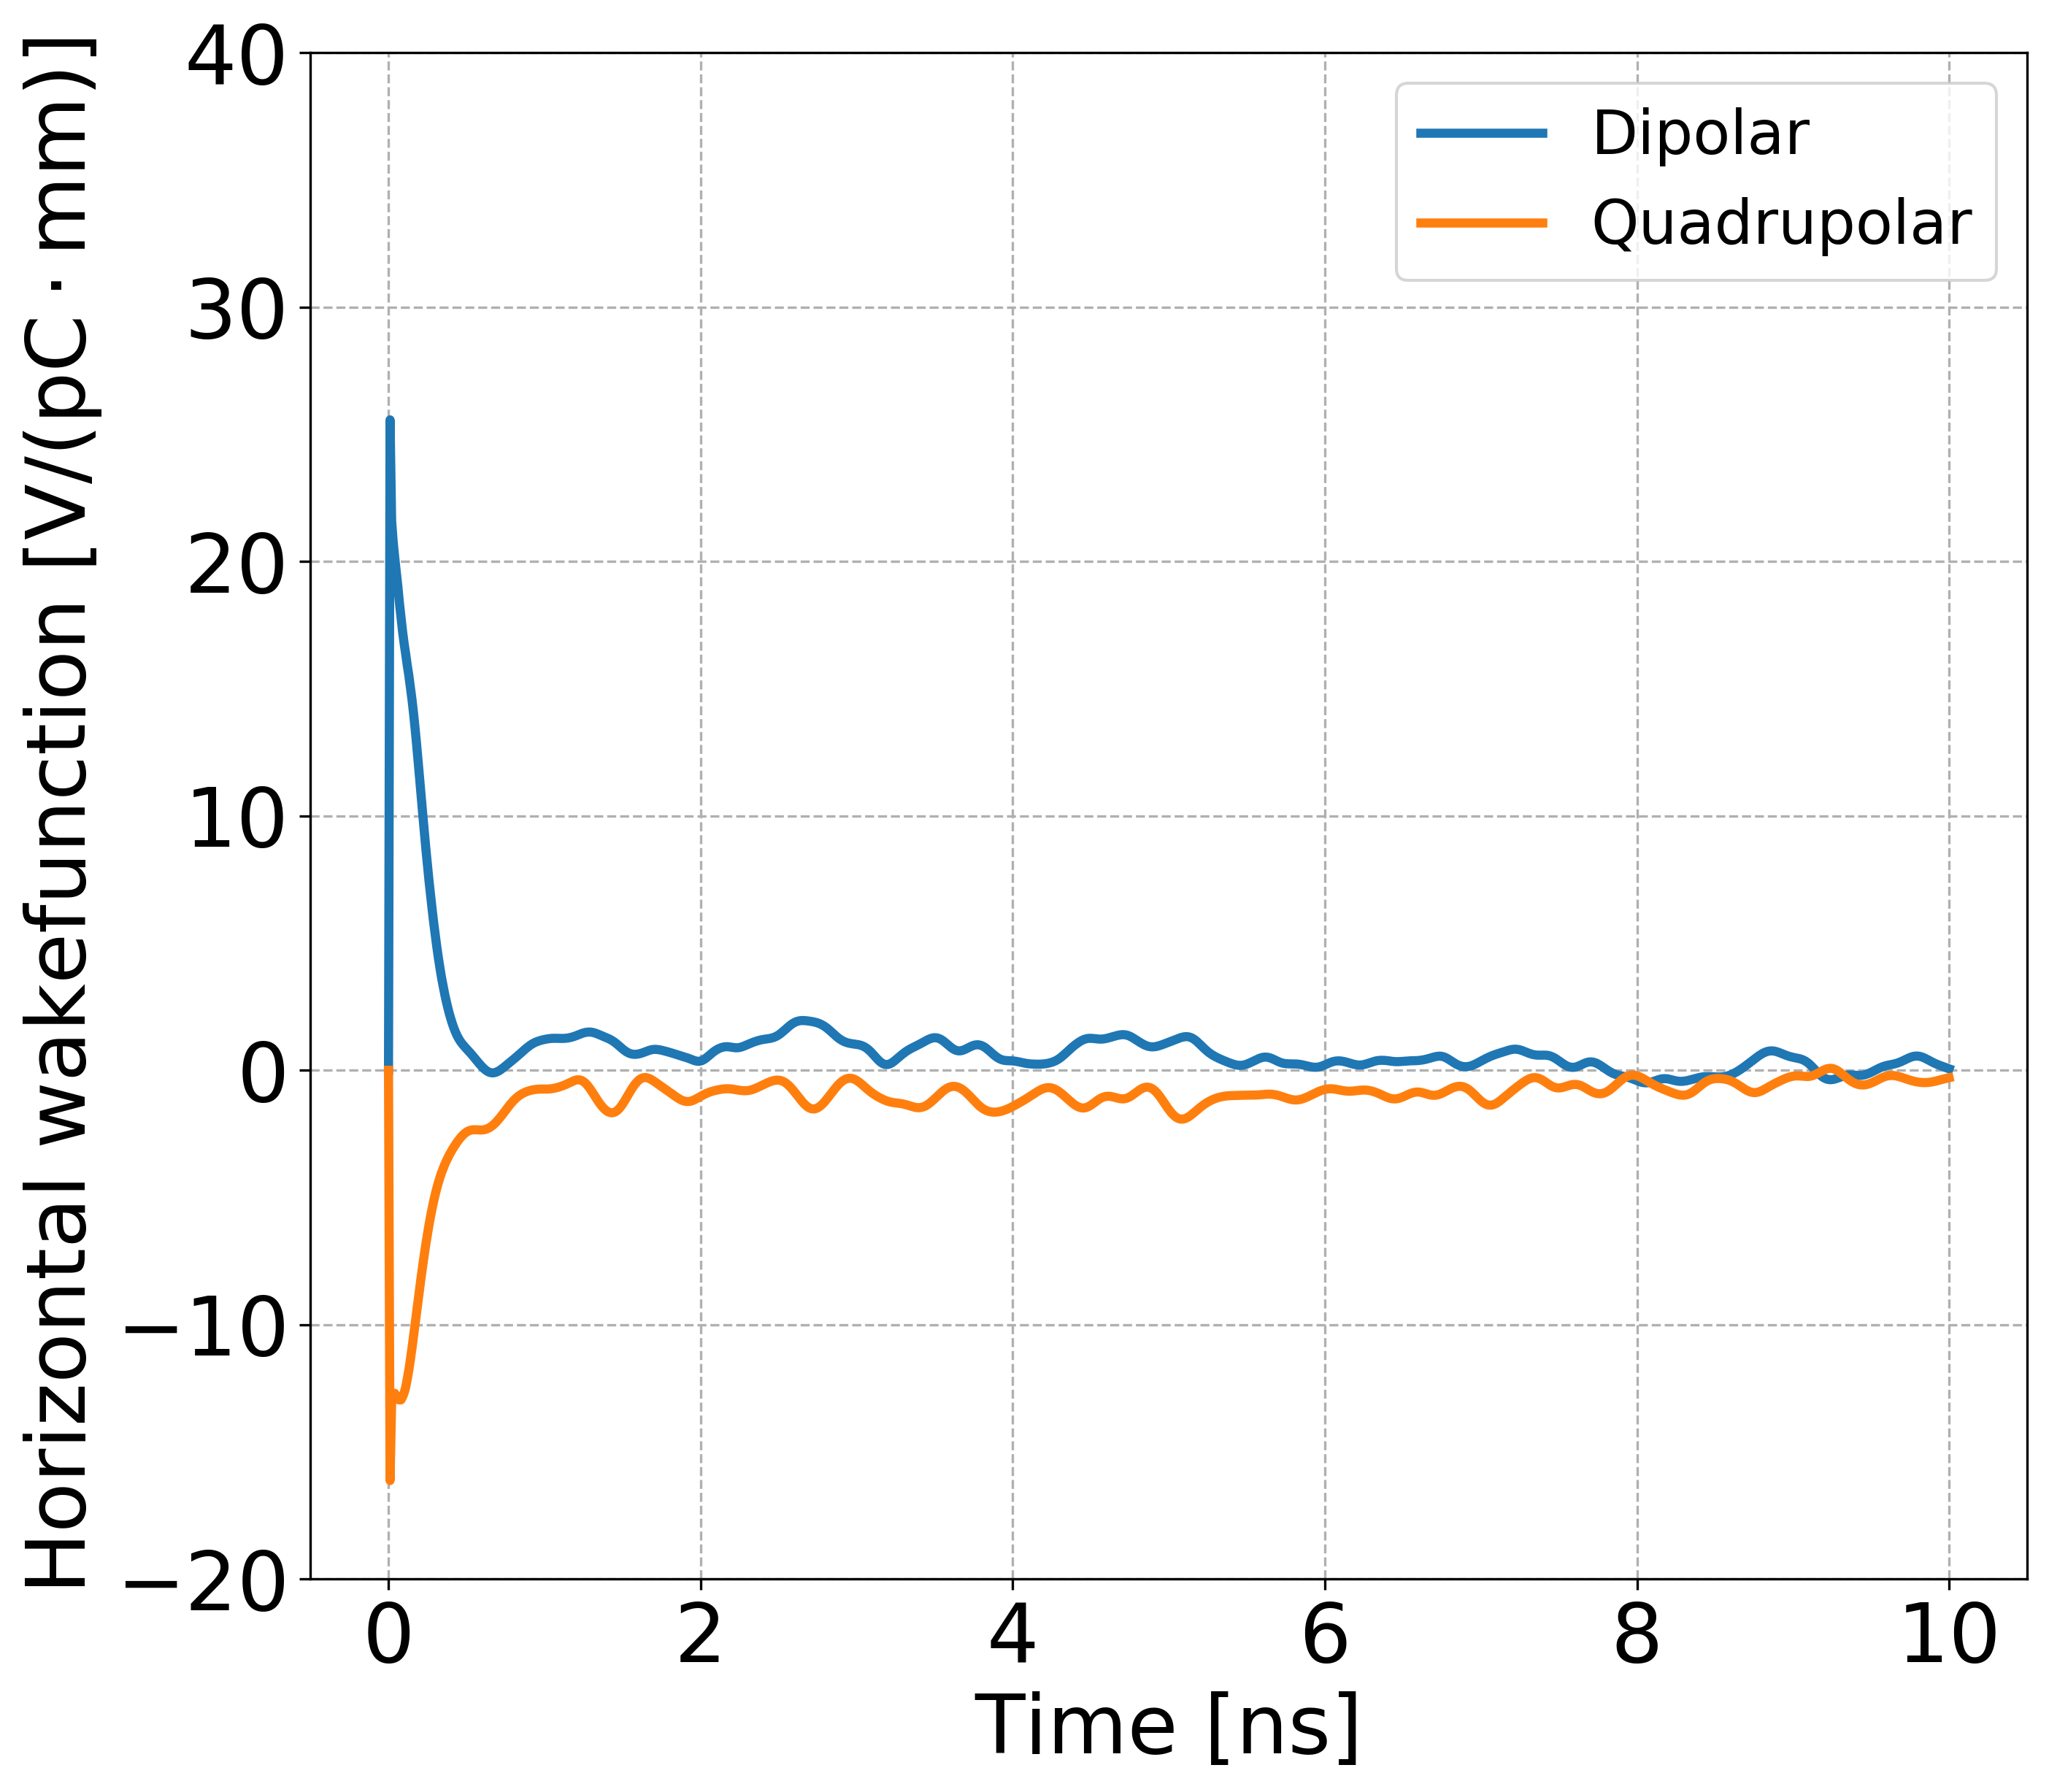
\includegraphics[width=1\textwidth]{images/Ch7/Q26_complete_SPS_model_wakefunctions_H_plane.png}
        %\caption{$y=\sin(2 \pi f t),\ f=50$ Hz}
        %\label{fig:add_label_here}
    \end{subfigure}
    \hfill
    \begin{subfigure}[t]{0.45\textwidth}
        \centering
        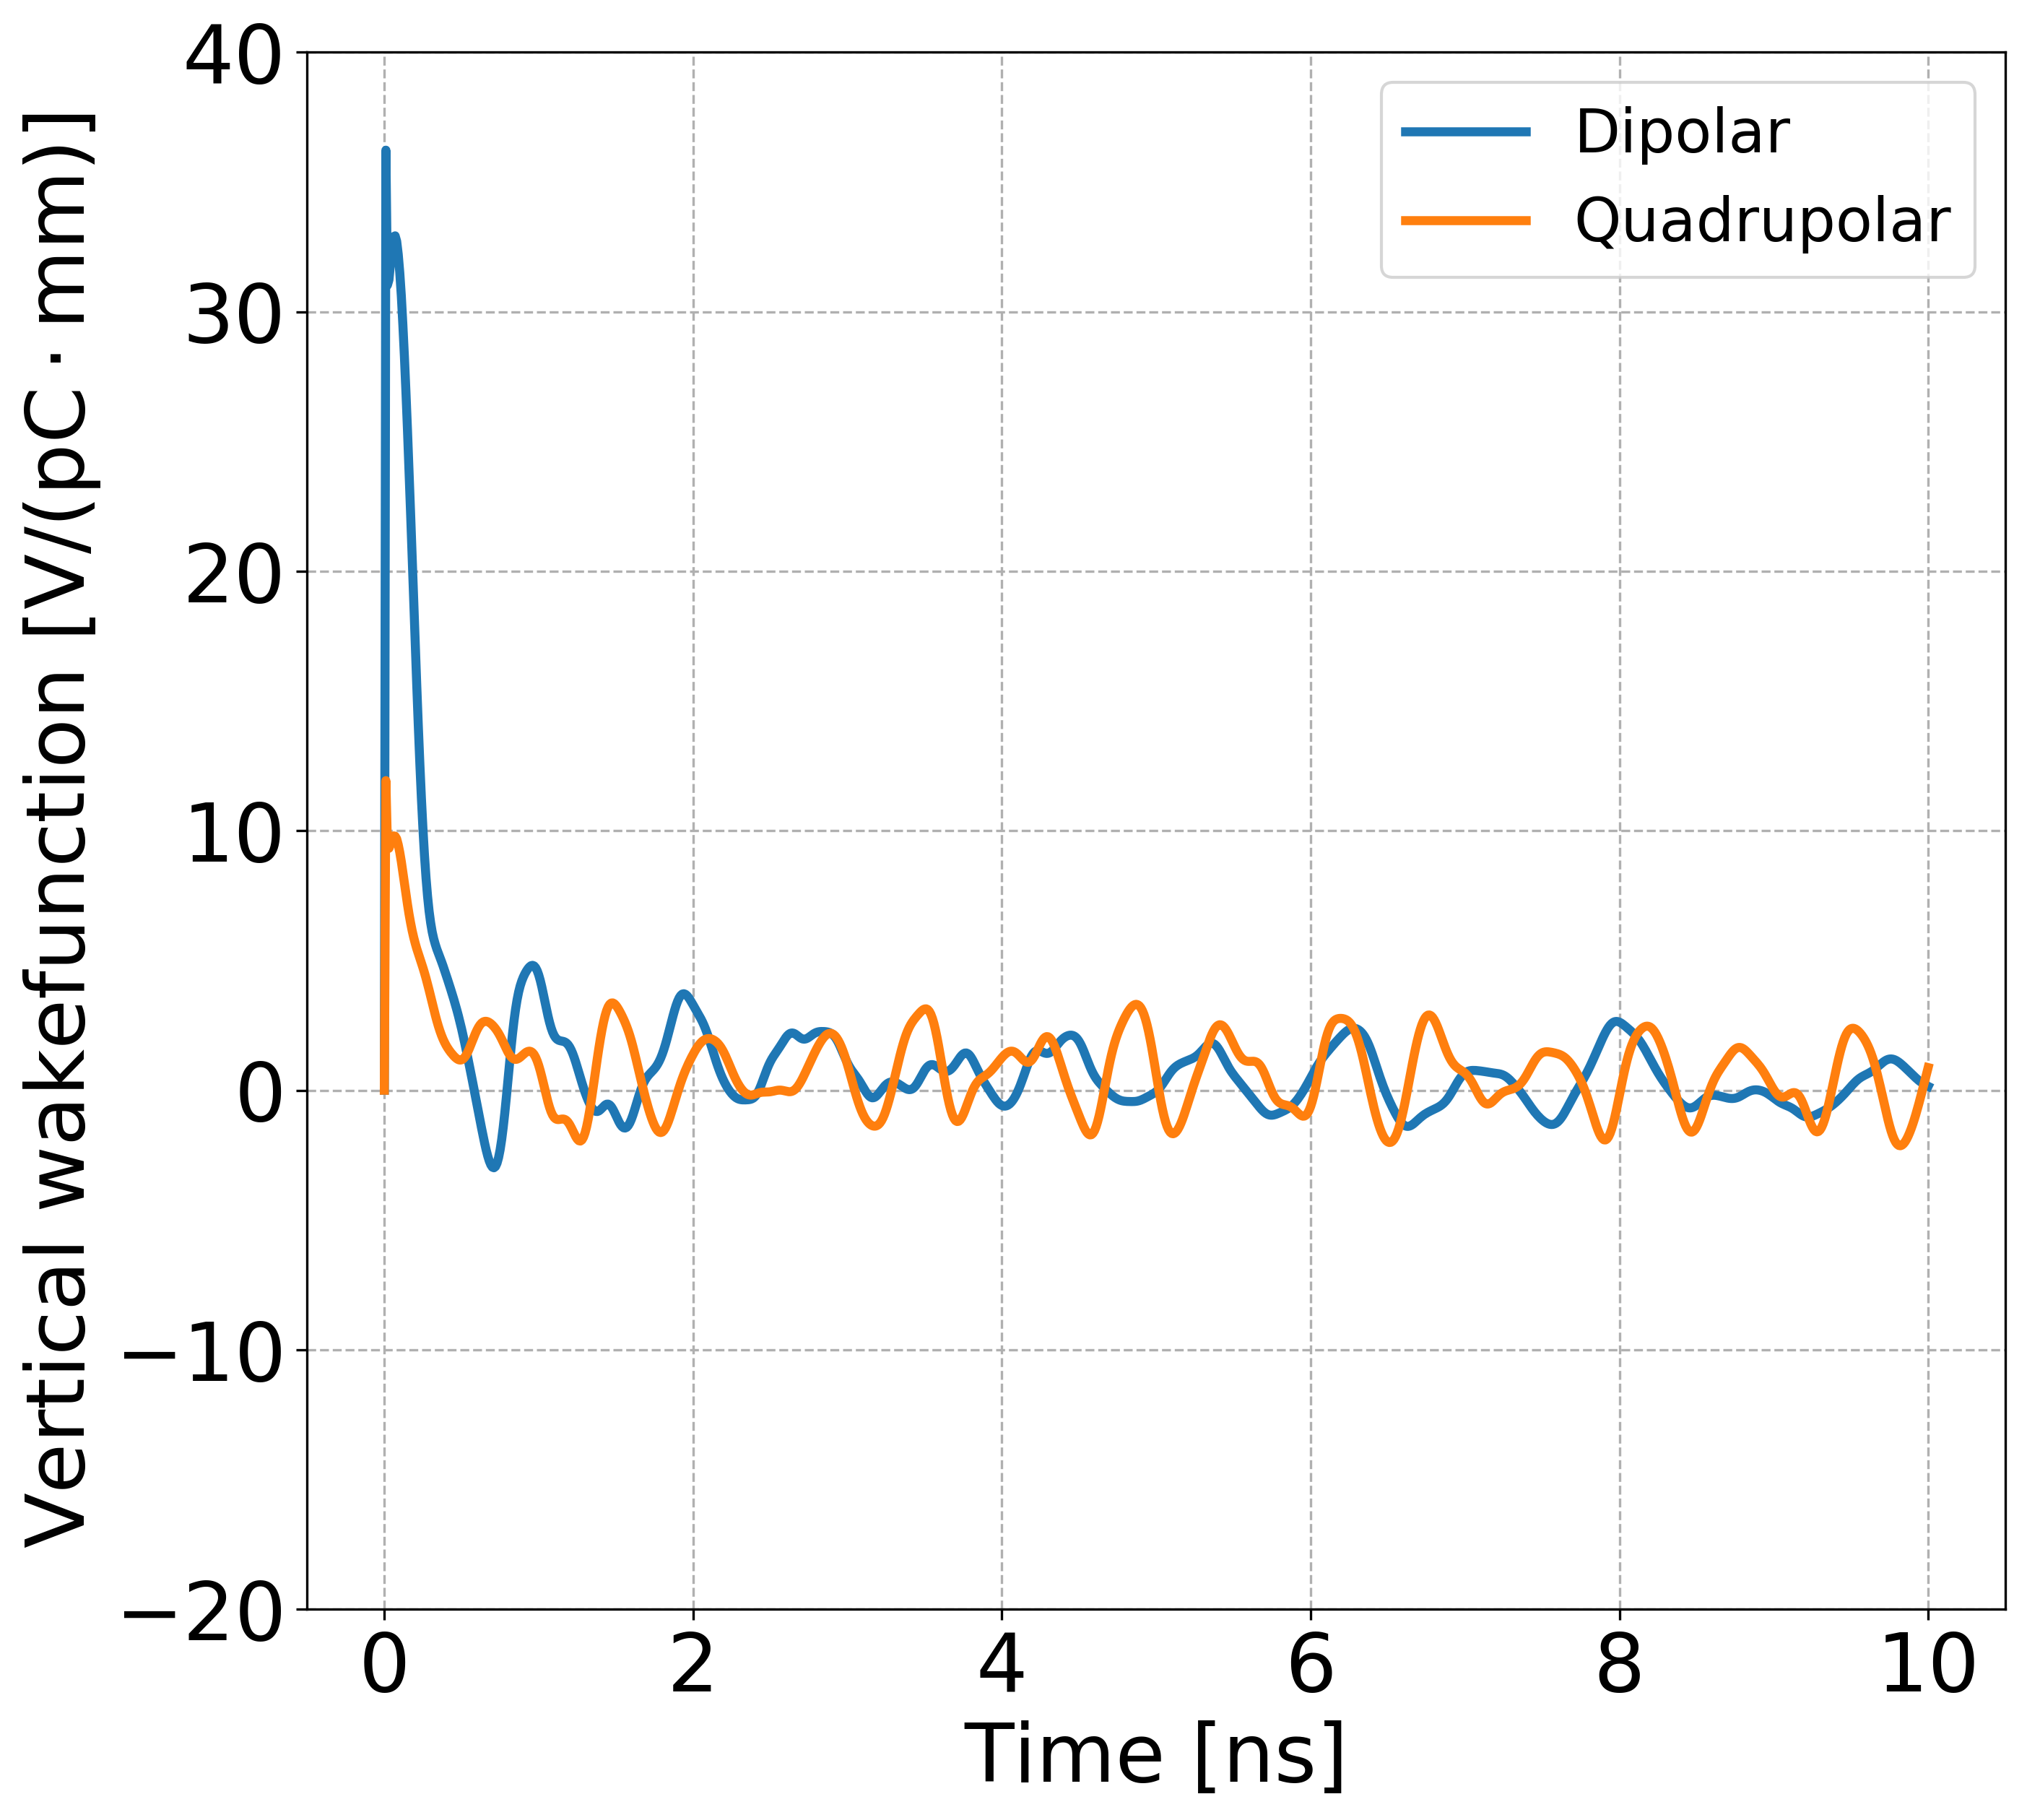
\includegraphics[width=1\textwidth]{images/Ch7/Q26_complete_SPS_model_wakefunctions_V_plane.png}
        %\caption{Discrete Fourier transform}
        %\label{fig:add_label_here}
    \end{subfigure}
    \hfill
     \caption{Horizontal (left) and vertical (right) wakefunctions of the SPS. The wake functions are available in the public gitlab repository of Ref.~\cite{sps_impedance_model_git}. For comparison the bunch length in the SPS CC experiments is $\sim$ 1.85\,ns (4$\mathrm{\sigma_t}$).} % bunch passage
     \label{fig:sps_wakefunctions_model_H_V}
 \end{figure}


% slide 9 https://accelconf.web.cern.ch/ipac2019/talks/weypls1_talk.pdf

% Carlo Zaninni thesis: s, it is important to have an accurate description of the wake at a distance z significantly smaller than the RMS bunch-length, which means that the impedance calculation needs to be accurate up to very high frequency (depending on the accelerator we consider, from a few GHz to the range of THz). 

\subsection{Coherent tune shift with intensity and growth rate}
- growth rate of mode 0
- shift of mode 0
One of the properties which is also used for checking the correct implemetation of the model. which as we will say later on is relevant to the suppression mechanism is the coherent tune shift with 

- model benchmarked but not as thorough for ... not gor single bunhces at that low intensity?

- we figured out


\section{Simulations setup}

In this section, the setup of the PyHEADTAIL simulations that were performed to study the impact of the beam coupling impedance on the emittance growth due to $\CC$ RF noise is described. The relevant machine and beam parameters are summarised in Table~\ref{tab:sps_pyheadtail_emit_growth_parameters}. The optics parameters were extracted from the SPS design parameters (nominal model for Q26 optics: Section~\ref{subsec:SPS_optics_model}), excpet for the vertical alpha function at the location of the CC2, $\alpha_{y, CC2}$ which is set to zero for simplicity as its value doesn't affect the emittance evolution. \textcolor{red}{Maybe elaborate a bit more on why it doesn't affect it?}. The rest of the lsited parameters are very similar to the experimental conditions during the emittance growth measurmentes of 2018 (discussed in Chapter~\ref{Ch:2018_analyisis}).


\normalsize{\textbf{Crab Cavity RF noise levels}}\\
\normalsize{\textbf{Amplitude detuning}}\\
\normalsize{\textbf{Parameters particularly for simulations without imepdance effects}}\\
\normalsize{\textbf{Parameters particularly for simulations with imepdance effects}}\\


The parameters used for the simulations were

imulations used the SPS design parameters and the beam conditions as in the experiment of 2018.

Table with parameters, including macroparticles number + slices + average beta funtion for convinience.



\begin{table}[!hbt]
	\begin{minipage}{\textwidth}
      \begin{centering}
   \caption{Relevant machine and beam parameters used to study the impact of the beam transverse impedance on the emittance evolution due to CC RF noise with the PyHEADTAIL code.}
	\begin{tabu} to \textwidth {X[c,m] X[0.5c,m] X[0.5c,m] X[0.01c,m]}
		&&& \\[-6mm]
		\toprule \toprule
		\multicolumn{2}{l}{\textbf{Parameter}} &
		\multicolumn{2}{c}{\textbf{Value}} \\
		\bottomrule
      \multicolumn{2}{l}{Beam energy, $\symE$} & \multicolumn{2}{c}{270\,GeV} \\
      \multicolumn{2}{l}{Number of protons per bunch, $\Nb$} & \multicolumn{2}{c}{3 $\times 10^{10}$ p/b} \\
      \multicolumn{2}{l}{Horizontal / Vertical betatron tune, $\Qx$ / $\Qy$}  & \multicolumn{2}{c}{26.13 / 26.18} \\
      \multicolumn{2}{l}{Horizontal / Vertical first order chromaticity, $\Qpx$ / $\Qpy$}  & \multicolumn{2}{c}{1 / 1} \\
      \multicolumn{2}{l}{Main RF voltage / frequency,  $\VRF$ / $\fRF$}  & \multicolumn{2}{c}{5.088\,MV / 200.39\,MHz} \\ %200.3945
      \multicolumn{2}{l}{Synchrotron tune, $\Qs$}  & \multicolumn{2}{c}{0.0051} \\
      \multicolumn{2}{l}{$\CC 2$ voltage / frequency, $\VCC $ / $\fCC$}  & \multicolumn{2}{c}{1\,MV / 400.78\,MHz} \\
      \multicolumn{2}{l}{Vertical beta function at $\CC 2$, $\beta_{y, CC2}$}  & \multicolumn{2}{c}{73.82\,m} \\
      \multicolumn{2}{l}{Vertical alpha function at $\CC 2$, $\alpha_{y, CC2}$}  & \multicolumn{2}{c}{0\,m} \\
      \multicolumn{2}{l}{Vertical dispersion at $\CC 2$, $D_{y, CC2}$}  & \multicolumn{2}{c}{0\,m} \\
      \multicolumn{2}{l}{Number of bunches}  & \multicolumn{2}{c}{1} \\
      \multicolumn{2}{l}{Rms bunch length, 4$\sigmat$}  & \multicolumn{2}{c}{1.8 \,ns$^\ast$}\\
      \multicolumn{2}{l}{Horizontal / Vertical normalised emittance, $\emitx$ / $\emity$}  & \multicolumn{2}{c}{2\,$\mathrm{\mu m}$ / 2\,$\mathrm{\mu m^\ast}$}\\
      \multicolumn{2}{l}{Horizontal / Vertical rms tune spread, $\Dqxrms$ / $\Dqyrms$}  & \multicolumn{2}{c}{2.02 $\times 10^{-5}$ / 2.17 $\times 10^{-5}$ $^\dagger$}\\
      \bottomrule
	\end{tabu}
   \label{tab:sps_pyheadtail_emit_growth_parameters}
   \end{centering} \footnotesize{$^\ast$ Initial values at the beginning of the tracking.\\$^\dagger$ Here the rms betatron tune spread includes only the contribution from the detuning with amplitude present in the SPS machine. More details along with the calulcations for the listed values can be found in Appendix~\ref{app:detuning_with_amplitude}.}
   \end{minipage}
\end{table}





\section{First observations of emittance growth suppression by the impedance}


\section{Characterisation of the emittance growth suppression by the impedance}
